\section{Cross-Language Experience for Current Cooperative Games}

% To understand how language boundary affect cooperative game experience, we recruit 9 Taiwaneses and 3 Japaneses and divided into 2 separate group-types(i)Taiwan-Taiwan, (ii)Taiwan-Japan. We have validated that Taiwanese players don’t understand Japanese and vise versa. We choose three different cooperative games on Steam[1] (so that player can talk to each other through Steam Talk), Rocketbirds:Hardboiled Chicken(Cooperative Action Game) ,Portal 2 (Cooperative Puzzle Game), Monaco (Cooperative Stealth Game).To emulate quick match via Internet, two players are playing these games at two distinct rooms using headphones for communication. Players play these three games 30 minutes for each. After playing each game, players will fill up an eSFQ[2] questionnaire for rapid assessment of game experiences and conduct an open-ended interviews.

To understand how language barrier affects the cooperative experience for current games, we conducted a 12-person user study where half the participants shared common languages and half did not. 

\subsection{Study Design}

We recruited 3 Japanese speakers and 9 Taiwanese speakers, and confirmed that none of the Taiwanese speakers understood Japanese and vice versa. 3 pairs of the participants did not have a common language (Japanese-Taiwanese) and 3 pairs did (Taiwanese).

We selected 3 popular cooperative games currently on the market that had distinct gameplay and cooperation needs. Also, all three games supported real-time voice chat. 
\begin{enumerate}
    \item Rocketbirds - Hardboiled Chicken: a cooperative action game, in which players shoot enemies with different weapons.
    
    \item Portal 2: a cooperative puzzle game, in which players can create portals that teleport players and must use them intelligently to solve the puzzles.
    
    \item Monaco: a cooperative stealth game, in which players can evade guards, collect coins, and ecsape.
\end{enumerate}

In order to simulate cooperative gameplay over the Internet, pairs of players were placed in two different rooms and used headsets to communicate with each other. Participants played each of the three games for 30 minutes, and filled out an eSFQ\cite{eSFQ} questionnaire after each game. We also conducted open-ended interviews to understand their gaming experience at the end of the sessions. 



\subsection{Results}

\begin{figure}[!t]
\centering
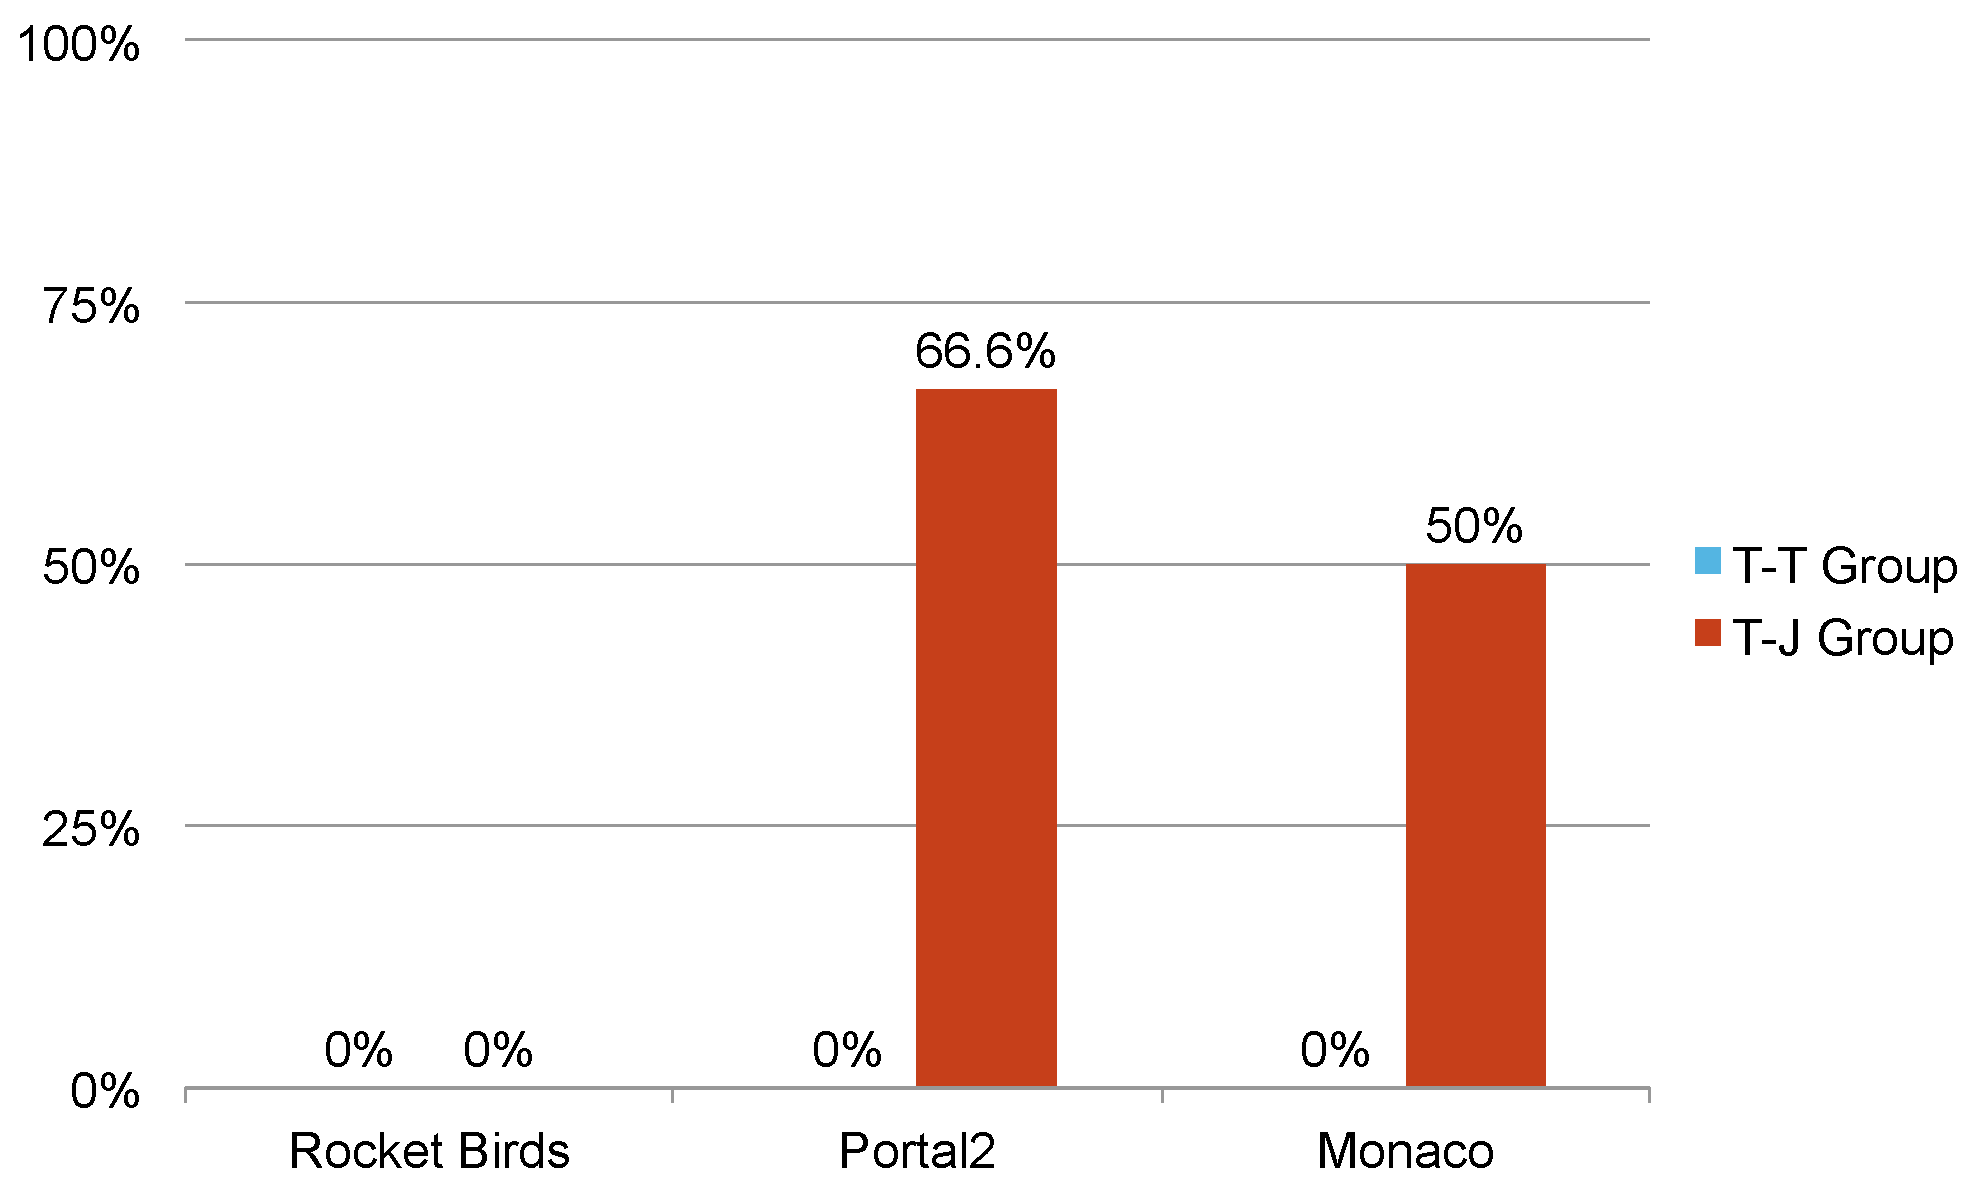
\includegraphics[width=0.9\columnwidth]{Figures/PS_Frus.pdf}
\caption{The eSFQ Frustration index, which is the percentage of players who reported a frustrating experience, of three cooperative games for players \textit{with} and \textit{without} common languages.}
\label{fig:PS_Frus}
\end{figure}

\begin{figure}[!t]
\centering
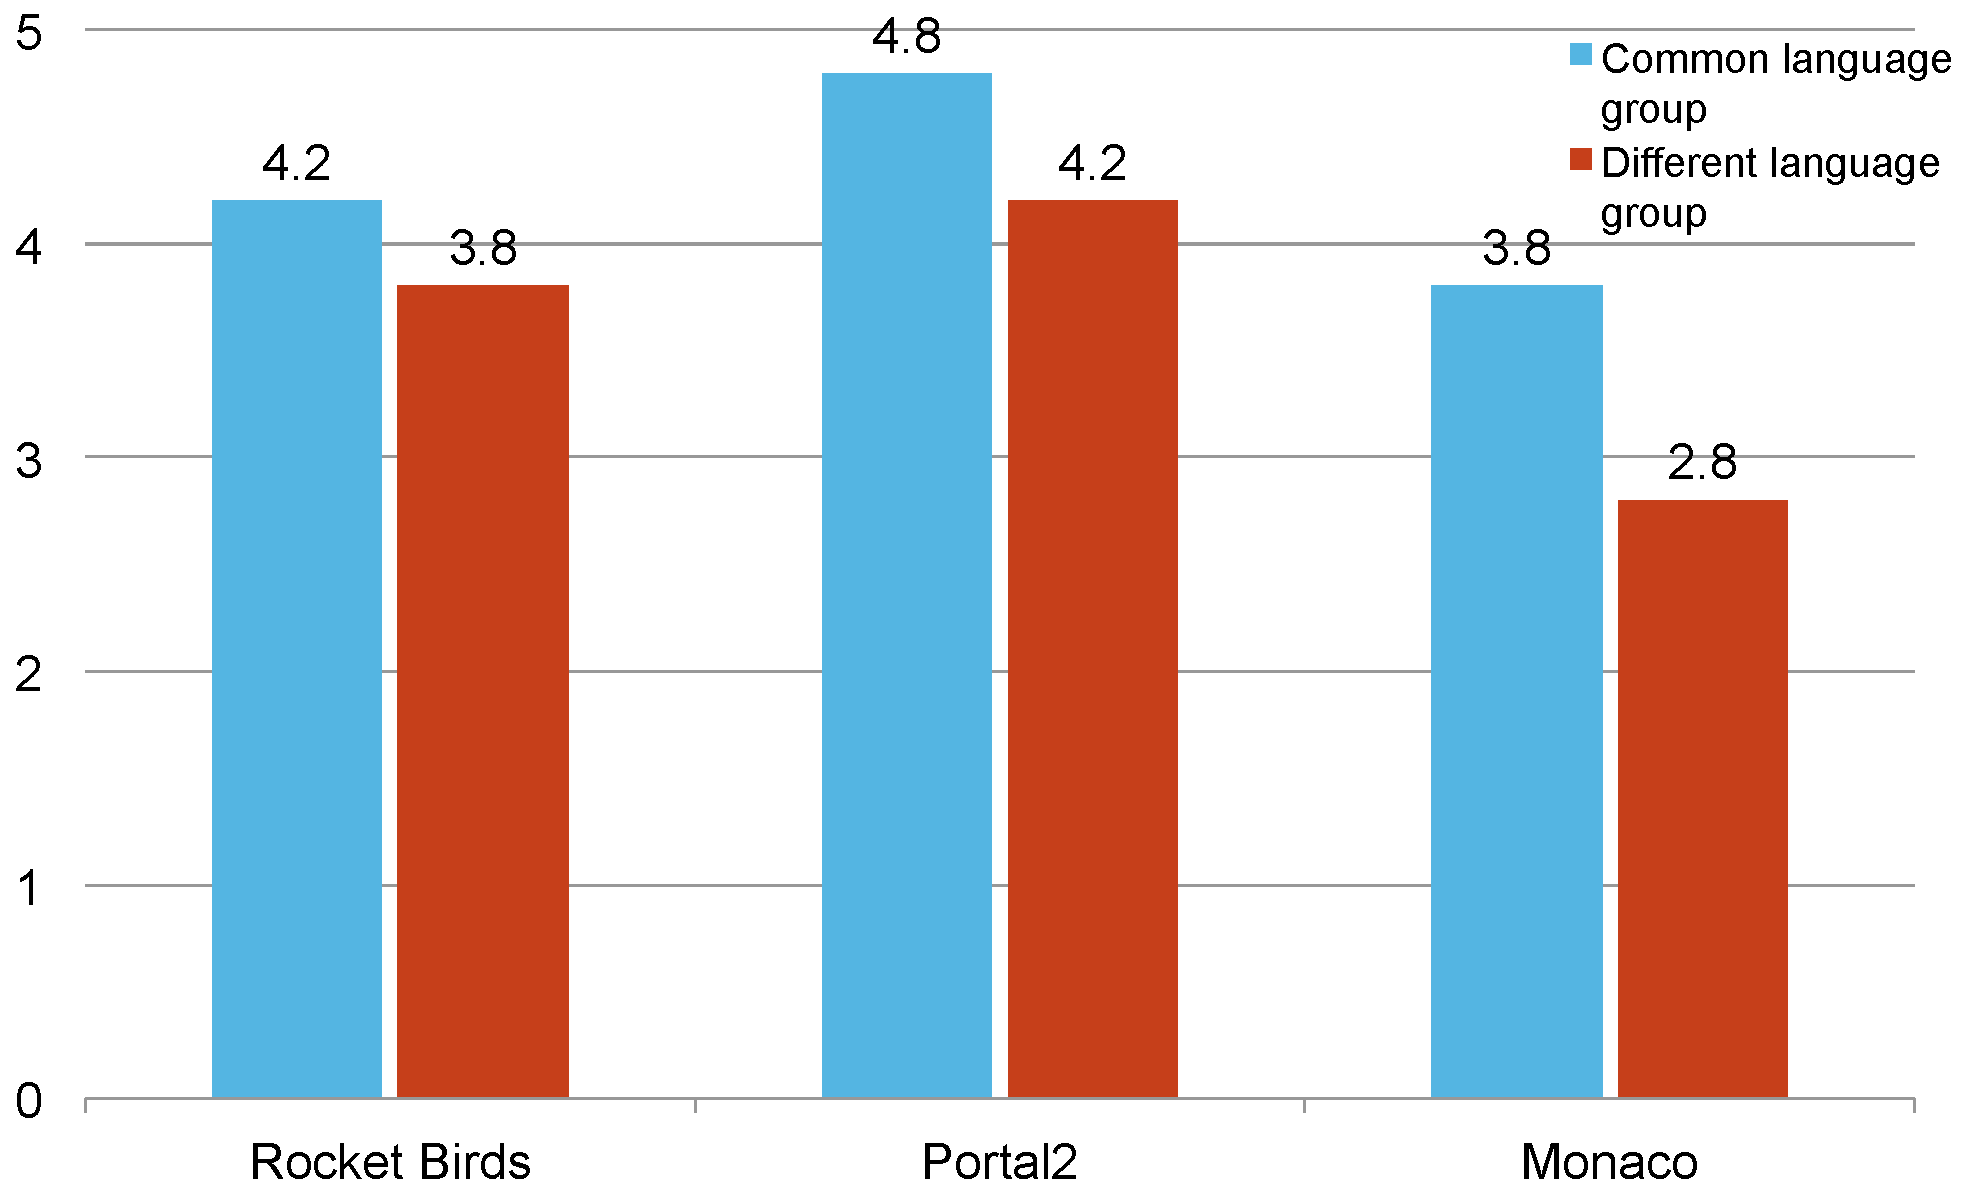
\includegraphics[width=0.9\columnwidth]{Figures/PS_FunAndEnj.pdf}
\caption{The eSFQ Fun and Enjoyment rating (on a scale of 1 to 5) of three cooperative games for players \textit{with} and \textit{without} common languages.}
\label{fig:PS_FunAndEnj}
\end{figure}

% 1. frustraing 比較,
% 2. fun enj 下降

Figure~\ref{fig:PS_Frus} shows the eSFQ Frustration index, which is the percentage of players who reported the experience as frustrating, for players \textit{with} and \textit{without} common languages.
For two out of the three games, Portal 2 and Monaco, frustration is significantly higher for players without common languages than than those who did. In fact, none of the players with a common spoken languages reported any of the games as frustrating. 

Figure~\ref{fig:PS_FunAndEnj}, shows the average eSFQ Fun and Enjoyment rating for each game (on a scale of 1 to 5), for players \textit{with} and \textit{without} common languages. The rating was lower for all three games when the players did not have common languages. Overall, the Fun and Enjoyment rating was 3.6 vs 4.3 for players without common languages compared to those who could communicate using a common spoken language.

%\subsection{Discussion}
% \begin{figure}[!h]
% \centering
% 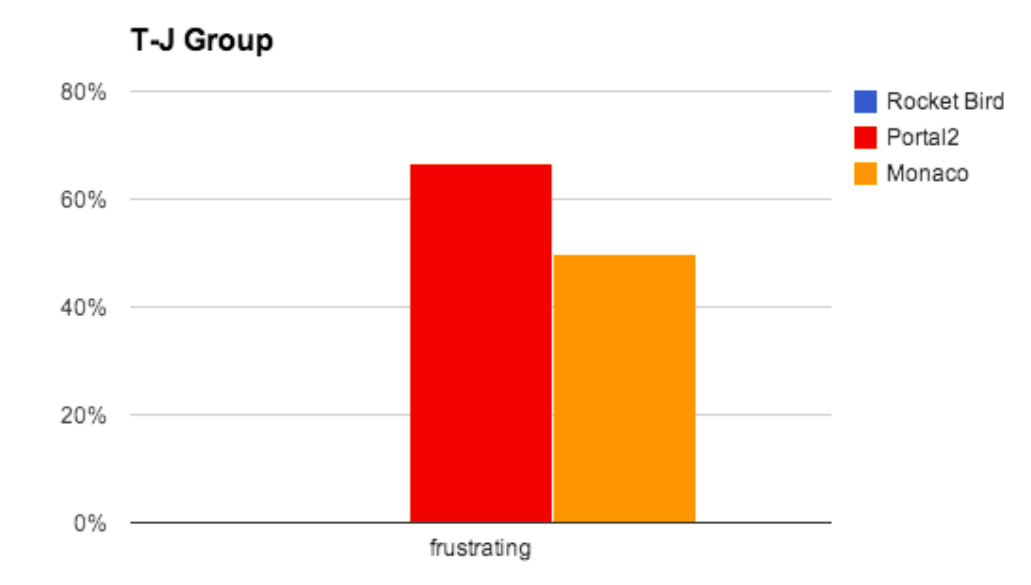
\includegraphics[width=0.9\columnwidth]{Figures/PS_F1.png}
% \caption{Frustrating index of eSFQ}
% \label{fig:figure1}
% \end{figure}

\subsection{Discussion}
% According to our study result, There is language boundary issue while playing Rocket Chicken,but it doesn’t cause frustrating and affect game experience significantly. We think this is because there are no complex concept to transmit. The main gameplay is dodging and shooting, players don’t need high-level-feature communication in this game.

The Rocketbirds' gameplay mainly consists of dodging and shooting, and required the least communication outside the game. As player P5 commented (shown in Table 1): ``We couldn't talk to each other, but communicated through moves and jumps.'' 
None of the players reported Rocketbirds as frustrating, and language barriers had the least effect on its fun and enjoyment rating as well.

%\subsubsection{Portal 2}
% Portal2 is reported the most frustrating while playing with different language players. Interview shows that language boundary really obstruct the process of gameplay and causing frustrating. We think it is because that,the main gameplay in portal 2 is solving complex puzzles, and it is impossible to pass the level with only one player, high-level-feature communication is required ,but it is hard to accomplish while playing with different language speaker.

Portal 2 was reported as the most frustrating by players without common languages. Portal 2's primary gameplay is to solve complex puzzles, which requires precise collaboration between the two partners. As some of the players mentioned: ``I couldn't tell what my partner was trying to do without talking to each other.''(P5), and ``It was tiring because it was hard to express my ideas.'' (P4),


%\subsubsection{Monaco}
% Monaco is reported not cooperative at all and highly frustrated. In our observation, different language group player only try to communicate at first and give up communicating really quickly, because this game is not restrict to single solution and forcing player to cooperate together. Even though two players are not cooperative working, single player can still stealth in the building and finish his mission, but the difficulty will significantly increase. We think this cause the game frustrating and players think this game is not cooperative at all.

Monaco's gameplay allowed a single player to solve a challenge, although cooperation would make it significantly easier. Player P4 mentioned: ``I didn't know where the exit was, and my partner couldn't tell me.'', yet P9 stated:  ``This game is simple. We didn't really need any communication with each other.''

%, is reported not cooperative at all and frustrated while playing the game. In our observation, different language group players only try to communicate at first, and then give up to communicate with each other quickly. The reason is that Monaco is not restricted to a single solution to the challenge and force players to cooperate together. Under this gameplay environment, asingle player can still finish his own mission secretly in the building, even though both players are not cooperative working and then the difficulty will increase significantly. We consider that this situation would make the gameplay experience be frustrated and players would think this game does not need to cooperate at all.



\begin{table}[!h]
% \renewcommand\arraystretch{1.2}
  \centering
  \begin{tabular}{
  !{\vrule width2pt}c
  %!{\vrule width2pt}m{0.7\columnwidth}
  !{\vrule width2pt}p{0.7\columnwidth}
  !{\vrule width2pt}c}
    \Xhline{2px}
    \tabhead{Game} &
    \multicolumn{1}{p{0.7\columnwidth}!{\vrule width2pt}}{\tabhead{Feedback from Players without Common Languages}} \\
    \Xhline{2px}
    Rockebirds & 
    \begin{itemize}
	  \item ``Although it was slower without talking, the challenges could still 
    be beaten with patience.''(P2)
%    \item ``We couldn't discuss who needed help.''(P4)
    \item ``We couldn't talk to each other, but communicated through moves and jumps.''(P5)
	  \end{itemize}
    \\
    \Xhline{2px}
    Portal 2 & 
    \begin{itemize}
    \item ``It was tiring because it was hard to express my ideas.''(P4)
    \item ``I couldn't tell what my partner was trying to do without talking to each other.''(P5)
    %\item ``I could't understand what my partner was saying, but guessed by his movement.''(P6)
    \end{itemize}
    \\
    \Xhline{2px}
    Monaco & 
    \begin{itemize}
    \item ``I didn't know where the exit was, and my partner couldn't tell me.''(P4)
    \item ``This game is simple. We didn't really need any communication with each other.''(P9)
    \end{itemize}
    \\
    \Xhline{2px}
  \end{tabular}
  \caption{Interview comments by players without common languages.}
  \label{tab:table1}
\end{table}



